\paragraph{Faraday効果}
磁場が電気的な応答に影響を与えることは一般によく知られている.物質の光応答に磁気が寄与するものを,「磁気光学効果」という.
今回はその中の一つであるFaraday効果について見ていこう.
Faraday効果とは,\textbf{直線偏光が磁化している物体中を通ったときに傾いた楕円偏光となる}現象である.
直線偏光とは位相,振幅が等しい円偏光が重なってできているものと考えることができる.

物質の中を電磁波が伝播するときは,一般にそのエネルギーは散逸し,振幅は減衰する.
その度合いを消失係数$\kappa$で表す.また,\textbf{物質中を伝わる電磁波の減衰は距離の指数関数で表される}.
これをLambert-Beerの法則という.よって,物質中で$x$だけ進んで,振幅が$A$倍になったときに
\begin{align}
  A=\exp\left( - \dfrac{\kappa\omega{x}}{c}\right)
\end{align}
で消失係数$\kappa$を定義する.屈折率$n$の物質中で電磁波が$x$伝わった時の電場は,
\begin{align}
  \boldsymbol{E}=\boldsymbol{E}_0\exp\left( - \dfrac{\kappa\omega{x}}{c}\right)\exp\left[ - i\omega\left(t - \dfrac{x}{c/n}\right)\right] = \boldsymbol{E}_0\exp\left[ - i\omega{t}+i\dfrac{\omega{x}}{c/N}\right]
  \label{faraday_eff_E_x}
\end{align}
で表される.$x=0$での振幅を$\boldsymbol{E}_0$とする.ここで,複素屈折率$N$
\begin{align}
  N=n+i\kappa
\end{align}
を導入した.
この$N$によって,位相変化の項の中に減衰も含めることができるのだ.
まず,\eqref{faraday_eff_E_x}にならって,電場,磁場をそれぞれ
\begin{align}
  \boldsymbol{E} &= \boldsymbol{E}_0\exp\left[i(\boldsymbol{K}\cdot\boldsymbol{r} - \omega{t})\right]\label{faraday_eff_Edef}\\
  \boldsymbol{H} &= \boldsymbol{H}_0\exp\left[i(\boldsymbol{K}\cdot\boldsymbol{r} - \omega{t})\right]\label{faraday_eff_Hdef}
\end{align}
とする.ただし,$\boldsymbol{K}$は複素波数ベクトルで,真空中の波数ベクトルを$\boldsymbol{k}$とすると,
\begin{align}
  \boldsymbol{K}=N\boldsymbol{k}\label{faraday_eff_K}
\end{align}
の関係がある.物質の比誘電率テンソルを$\tilde{\varepsilon}$とすると,等方的な物質の電気感受率テンソルの形から,
\begin{align}
  \tilde{\varepsilon}=
  \dfrac{1}{\varepsilon_0}
  \left(
  \begin{array}{ccc}
    \varepsilon_{\xi\xi} & \varepsilon_{\xi\eta} & 0 \\
    - \varepsilon_{\xi\eta} & \varepsilon_{\xi\xi} & 0 \\
    0 & 0 & \varepsilon_{\zeta\zeta}
  \end{array}
  \right)
  \label{faraday_eff_tensor}
\end{align}
となる.よって,Maxwell方程式は,
\begin{align}
  \rot \boldsymbol{E}= - \mu_0\dfrac{\partial\boldsymbol{H}}{\partial{t}} , \label{faraday_eff_rotE} \\
  \rot \boldsymbol{H}=\tilde{\varepsilon}\varepsilon_0\dfrac{\partial\boldsymbol{E}}{\partial{t}} . \label{faraday_eff_rotH}
\end{align}
\eqref{faraday_eff_rotE}と\eqref{faraday_eff_rotH}から$\boldsymbol{H}$を消去すると,
\begin{align}
  \rot \left(\dfrac{1}{\mu_0}\rot \boldsymbol{E}\right)=\tilde{\varepsilon}\varepsilon_0\dfrac{\partial^2\boldsymbol{E}}{\partial t^2} .
\end{align}
また,ベクトル解析の公式から,
\begin{align}
  \grad(\rot \boldsymbol{E}) - {\nabla}^2\boldsymbol{E}= - \tilde{\varepsilon}\dfrac{1}{c^2}\dfrac{\partial^2\boldsymbol{E}}{\partial t^2}
\end{align}
と変形できる.これに\eqref{faraday_eff_Edef}を代入すると,
\begin{align}
  - (\boldsymbol{E}\cdot\boldsymbol{K})\boldsymbol{K}+\boldsymbol{K}^2\boldsymbol{E}=\tilde{\varepsilon}\left(\dfrac{\omega}{c}\right)^2\boldsymbol{E} .  \label{faraday_eff_Ek}
\end{align}
$\boldsymbol{K}$と平行で,大きさが物質の複素屈折率$N$に等しい複素屈折率ベクトル$\boldsymbol{N}$を考える.
定義と\eqref{faraday_eff_K}から,
\begin{align}
  \dfrac{\boldsymbol{K}}{\omega}=\dfrac{\boldsymbol{N}}{c} . \label{faraday_eff_Ndef}
\end{align}
\eqref{faraday_eff_Ndef}を\eqref{faraday_eff_Edef}に代入すると,
\begin{align}
  \boldsymbol{E} &= \boldsymbol{E}_0\exp\left[i(\boldsymbol{K}\cdot\boldsymbol{r} - \omega{t})\right] \notag \\
  &= \boldsymbol{E}_0\exp\left[ - i\omega\left(t - \dfrac{\boldsymbol{N}\cdot\boldsymbol{r}}{c}\right)\right] . \label{faraday_eff_EN}
\end{align}
ここで,\eqref{faraday_eff_EN}を\eqref{faraday_eff_Ek}に代入すると,
\begin{align}
  N^2\boldsymbol{E} - (\boldsymbol{E}\cdot\boldsymbol{N})\boldsymbol{N} - \tilde{\varepsilon}\boldsymbol{E}=0 . \label{faraday_eff_NE}
\end{align}
光の進む向きは$\zeta$方向であるとする.つまり,
\begin{align}
  \boldsymbol{N}=(0,0,N) \label{faraday_eff_Nvec}
\end{align}
である.
\eqref{faraday_eff_tensor}と\eqref{faraday_eff_NE},\eqref{faraday_eff_Nvec}を合わせると,
\begin{align}
  \left(
  \begin{array}{ccc}
    N^2 - \varepsilon_{\xi\xi} &  - \varepsilon_{\xi\eta} & 0 \\
    \varepsilon_{\xi\eta} & N^2 - \varepsilon_{\xi\xi} & 0 \\
    0 & 0 &  - \varepsilon_{\zeta\zeta}
  \end{array}
  \right)
  \left(
  \begin{array}{c}
    E_\xi \\
    E_\eta\\
    E_\zeta
  \end{array}
  \right)
  =0
  \label{faraday_eff_equation}
\end{align}
となる.さらにこれは,
\begin{align}
  \left(
  \begin{array}{cc}
    N^2 - \varepsilon_{\xi\xi} &  - \varepsilon_{\xi\eta} \\
    \varepsilon_{\xi\eta} & N^2 - \varepsilon_{\xi\xi} \\
  \end{array}
  \right)
  \left(
  \begin{array}{c}
    E_\xi \\
    E_\eta
  \end{array}
  \right)
  =0
  \label{faraday_eff_equation1}\\
  - \varepsilon_{\zeta\zeta}E_{\zeta}=0 \label{faraday_eff_equation2}
\end{align}
と変形できる.\eqref{faraday_eff_equation2}より,
\begin{align}
  \varepsilon_{\zeta\zeta}=0
\end{align}
である.また,\eqref{faraday_eff_equation1}が$E_\xi=0$かつ$E_\eta=0$以外の解を持つためには,
\[
\left|
\begin{array}{cc}
  N^2 - \varepsilon_{\xi\xi} &  - \varepsilon_{\xi\eta} \\
  \varepsilon_{\xi\eta} & N^2 - \varepsilon_{\xi\xi} \\
\end{array}
\right|
=0
\]
であればよい.よって,
\begin{align}
  {N_\pm}^2=\varepsilon_{\xi\xi}\pm i\varepsilon_{\xi\eta} . \label{faraday_eff_Npm}
\end{align}
\eqref{faraday_eff_Npm}を\eqref{faraday_eff_equation1}に代入すれば,$N_+$では$iE_\xi=E_\eta$となり,\eqref{faraday_eff_Edef}と比較するとこれは左回りの円偏光である.
よって,
\begin{align}
  \Delta{N} &= N_+ - N_ - \notag \\
  &= \sqrt{\varepsilon_{\xi\xi}+i\varepsilon_{\xi\eta}} - \sqrt{\varepsilon_{\xi\xi} - i\varepsilon_{\xi\eta}}\notag \\
  &\sim\dfrac{i\varepsilon_{\xi\eta}}{\sqrt{\varepsilon_{\xi\xi}}}
\end{align}
この実部と虚部を取ると,
\begin{align}
  \Delta{n} &= \text{Re}\,(\Delta{N})\notag \\
  &= \dfrac{\kappa\varepsilon'_{\xi\eta} - n\varepsilon''_{\xi\eta}}{n^2+\kappa^2} \label{faraday_eff_deltan}
\end{align}
\begin{align}
  \Delta{\kappa} &= \text{Im}\,(\Delta{N})\notag \\
  &= \dfrac{n\varepsilon'_{\xi\eta}+\kappa\varepsilon''_{\xi\eta}}{n^2+\kappa^2} \label{faraday_eff_deltakappa}
\end{align}
ただし,$\sqrt{\varepsilon_{\xi\xi}}\sim N=n+\kappa i\,$(磁化がないときの複素屈折率)であることを用いた.磁化がないとき,等方的な物質の誘電率テンソルは,
\begin{align}
  \varepsilon=
  \left(
  \begin{array}{ccc}
    \varepsilon_{11} & 0 & 0 \\
    0 & \varepsilon_{11} & 0 \\
    0 & 0 & \varepsilon_{11}
  \end{array}
  \right)
\end{align}
となるので,これは誘電率$\varepsilon_{11}$の物質としてふるまう.比透磁率が1とすると,確かに上記の関係式が成り立つ.また,$\varepsilon'$は実部,$\varepsilon''$は虚部をあらわす.
さらに,物質中での光のふるまいは位相変化と振幅変化の有無を考えると,以下の$4$種類があることが分かる.
\begin{enumerate}
  \item 物質に入る前は光は直線偏光である.
  \item $\Delta{n}$は左回りの旋光と右回りの旋光に対する屈折率の差である.これは各旋光の位相差を作る.物質の中では円偏光となる.だが,物質を出ると元通り直線偏光となる.
  \item $\Delta{\kappa}$は左回りの旋光と右回りの旋光に対する吸収率の差である.これは各旋光の振幅差を作る.物質の中では軸が不変の楕円偏光となる.これを円二色性という.
  \item 一般には$\Delta{n}$と$\Delta{\kappa}$が存在する.物質の中を進みながら,楕円自体が回転する.この場合は,トロコイドを描く.物質を出ると,傾いた楕円偏光となる.
\end{enumerate}

\begin{figure}[ht]
  \centering
  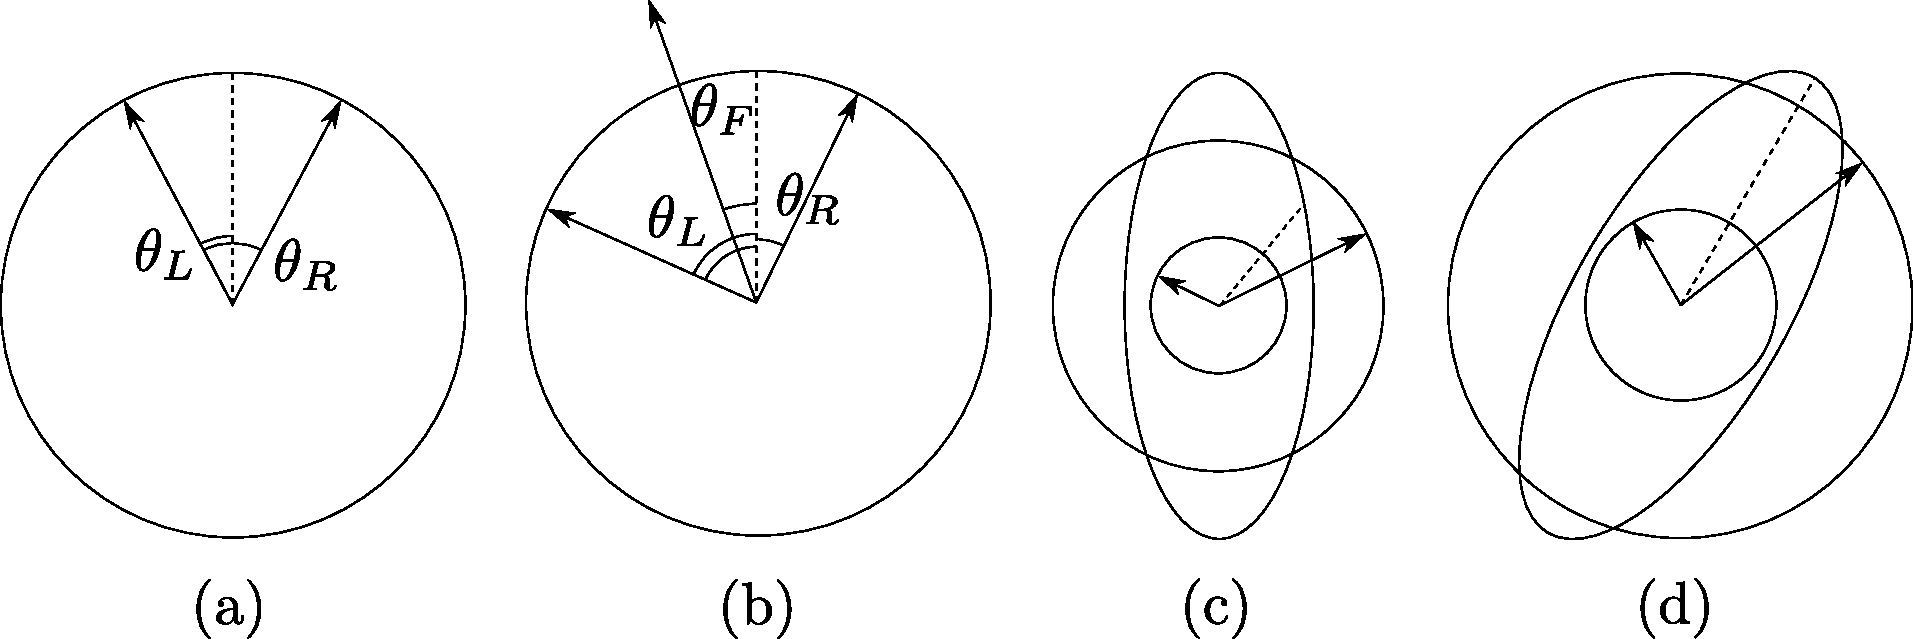
\includegraphics[scale=0.4]{faraday.pdf}
  \caption{}
  \label{faraday}
\end{figure}

物質中を$l$進んだ後の直線偏光の旋回角$\theta_F$は,
\begin{align}
  \theta_F &=  - \dfrac{\theta_R - \theta_L}{2}\notag \\
  &= \dfrac{2\pi(n_ -  - n_+)l}{2\lambda}\notag \\
  &=  - \pi\Delta{n}\dfrac{l}{\lambda} \label{faraday_eff_thetaF}
\end{align}
また,楕円偏光の楕円率(長軸と短軸の比)$\eta_F$は,
\begin{align}
  \eta_F &= \dfrac{E_L - E_R}{E_L+E_R}\notag \\
  &= \dfrac{\exp\left( - \dfrac{\kappa_+\omega{l}}{c}\right) - \exp\left( - \dfrac{\kappa_ - \omega{l}}{c}\right)}{\exp\left( - \dfrac{\kappa_+\omega{l}}{c}\right)+\exp\left( - \dfrac{\kappa_ - \omega{l}}{c}\right)}\notag \\
  &\sim  - \pi\Delta{\kappa}\dfrac{l}{\lambda} \label{faraday_eff_etaF}
\end{align}
となる.よって,\eqref{faraday_eff_deltan},\eqref{faraday_eff_deltakappa},\eqref{faraday_eff_thetaF},\eqref{faraday_eff_etaF}から,
\begin{align}
  \theta_F &=  - \dfrac{\omega}{2c}\cdot\dfrac{\kappa\varepsilon'_{\xi\eta} - n\varepsilon''_{\xi\eta}}{n^2+\kappa^2}l \\
  \eta_F &=  - \dfrac{\omega}{2c}\cdot\dfrac{n\varepsilon'_{\xi\eta}+\kappa\varepsilon''_{\xi\eta}}{n^2+\kappa^2}l
\end{align}
となる.
これは等方性媒質に対し,外部から磁場をかけて異方的にした効果である.

\paragraph{複素電磁波動方程式}
Faraday効果で複素屈折率という概念を導入した.振動子モデルでは複素感受率や複素誘電率である誘電関数も出てきた.
実数の物理量であった$n$,$\varepsilon$には,
\begin{align}
  \frac{c}{n}=\sqrt{\varepsilon\mu_0}
\end{align}
が成立し,さらに,電場に対しては波動方程式
\begin{align}
  \nabla^2\boldsymbol{E}=\varepsilon\mu_0\dfrac{\partial^2\boldsymbol{E}}{\partial{t}^2}
\end{align}
が成立した.

Faraday効果の項目で導入した複素物理量について復習しておく.
物質の中を電磁波が伝播するときは,一般にそのエネルギーは散逸し,振幅は減衰する.その度合いを消失係数$\kappa$で表す.
また,\textbf{物質中を伝わる電磁波の減衰は距離の指数関数で表される}.
これをLambert-Beerの法則という.よって,物質中で$x$だけ進んで,振幅が$A$倍になったときに
\begin{align}
  A=\exp\left(-\dfrac{\kappa\omega{x}}{c}\right)
\end{align}
で消失係数$\kappa$を定義する.屈折率$n$の物質中で電磁波が$x$伝わった時の電場は,
\begin{align}
  \boldsymbol{E}=\boldsymbol{E}_0\exp\left(-\dfrac{\kappa\omega{x}}{c}\right)\exp\left[-i\omega\left(t-\dfrac{x}{c/n}\right)\right] = \boldsymbol{E}_0\exp\left[-i\omega{t}+i\dfrac{\omega{x}}{c/N}\right]\label{comp_wave_eq_E}
\end{align}
で表される.$x=0$での振幅を$\boldsymbol{E}_0$とする.ここで,複素屈折率$N$
\begin{align}
  N=n+i\kappa
\end{align}
を導入した.
この$N$によって,位相変化の項の中に減衰も含めることができるのだ.
さらに,複素波数$K$を
\begin{align}
  \boldsymbol{K}=N\boldsymbol{k}=(n+i\kappa)\boldsymbol{k}
\end{align}
で定義する.この複素波数を用いると,(\ref{comp_wave_eq_E})は,
\begin{align}
  \boldsymbol{E}=\boldsymbol{E}_0\exp\left[i\left(\boldsymbol{K}\cdot\boldsymbol{r}-\omega{}t\right)\right]\label{comp_wave_eq_Ek}
\end{align}
と書くことができる.さらに,複素屈折率ベクトル$\boldsymbol{N}$を
\begin{align}
  \boldsymbol{N}=\dfrac{N}{k}\boldsymbol{k}\label{comp_wave_eq_def_N}
\end{align}
で定義すると,
\begin{align}
  \boldsymbol{E}=\boldsymbol{E}_0\exp\left[i\left(\dfrac{\omega}{c}\boldsymbol{N}\cdot\boldsymbol{r}-\omega{}t\right)\right]\label{comp_wave_eq_Eomega}
\end{align}
と書くこともできる.結局,
(\ref{comp_wave_eq_Ek}),(\ref{comp_wave_eq_Eomega})において,
\begin{quote}
  複素波数$\boldsymbol{K}$もしくは複素屈折率$N$の虚部が正だと減衰が起こる
\end{quote}
と言える.

複素数に対応する波動方程式は\eqref{comp_wave_eq_def_N}\eqref{comp_wave_eq_Eomega}から
\begin{align}
  \nabla^2 \boldsymbol{E} &= \left(\dfrac{i\omega{N}}{c}\right)^2 \boldsymbol{E}\\
  \dfrac{\partial^2\boldsymbol{E}}{\partial{t}^2} &= (i\omega)^2 \boldsymbol{E}
\end{align}
となる.これらから,減衰を複素屈折率として取り入れた電磁波動方程式
\begin{align}
  \nabla^2 \boldsymbol{E} = \left(\dfrac{1}{c/N}\right)^2\dfrac{\partial^2\boldsymbol{E}}{\partial{t}^2}\label{comp_wave_eq_comp_wave}
\end{align}
が導かれる.
振動子モデルで扱った散逸を無視しない誘電関数の形は,
\begin{align}
  \varepsilon(\omega)=\varepsilon_0\left(\dfrac{\varepsilon_{\text{b}}}{\varepsilon_0}+\dfrac{{\omega_p}^2}{{\omega_0}^2-\omega^2-i\gamma\omega}\right)\label{comp_wave_eq_permittivity}
\end{align}
となる.電荷分布や電流分布がないMaxwell方程式は,
\begin{align}
  \dive{\boldsymbol{E}}&=0\label{comp_wave_eq_dive}\\
  \text{rot}{\boldsymbol{E}}&=-\dfrac{\partial\boldsymbol{B}}{\partial{t}}\label{comp_wave_eq_rote}\\
  \text{rot}{\boldsymbol{B}}&=\varepsilon(\omega)\mu_0\dfrac{\partial\boldsymbol{E}}{\partial{t}}\label{comp_wave_eq_rotb}\\
  \dive{\boldsymbol{B}}&=0\label{comp_wave_eq_divb}
\end{align}
となる.(\ref{comp_wave_eq_dive}),(\ref{comp_wave_eq_rote}),(\ref{comp_wave_eq_rotb})から,
\begin{align}
  \nabla^2\boldsymbol{E}=\varepsilon(\omega)\mu_0\dfrac{\partial^2\boldsymbol{E}}{\partial{t}^2}
\end{align}
となる.これと(\ref{comp_wave_eq_comp_wave}),(\ref{comp_wave_eq_permittivity})から,
\begin{align}
  N &= n+i\kappa\notag\\
  &=\sqrt{1+\dfrac{{\omega_p}^2}{{\omega_0}^2-\omega^2-i\gamma\omega}}
\end{align}
となることが分かる.結局,複素数に拡張した電磁波動方程式は,
\begin{align}
  \nabla^2\boldsymbol{E} &= \left(\dfrac{\varepsilon_{\text{b}}}{\varepsilon_0}+\dfrac{{\omega_p}^2}{{\omega_0}^2-\omega^2-i\gamma\omega}\right)\varepsilon_0\mu_0\dfrac{\partial^2\boldsymbol{E}}{\partial{t}^2}\notag\\
  &= \left[n(\omega)^2-\kappa(\omega)^2+2in(\omega)\kappa(\omega)\right]\varepsilon_0\mu_0\dfrac{\partial^2\boldsymbol{E}}{\partial{t}^2}\label{comp_wave_eq_newequationE}
\end{align}
と書き直される.(\ref{comp_wave_eq_newequationE})は分散と減衰も考慮した式である.磁束密度に関する方程式も,
\begin{align}
  \nabla^2\boldsymbol{B} &= \left(\dfrac{\varepsilon_{\text{b}}}{\varepsilon_0}+\dfrac{{\omega_p}^2}{{\omega_0}^2-\omega^2-i\gamma\omega}\right)\varepsilon_0\mu_0\dfrac{\partial^2\boldsymbol{B}}{\partial{t}^2}\notag\\
  &= \left[n(\omega)^2-\kappa(\omega)^2+2in(\omega)\kappa(\omega)\right]\varepsilon_0\mu_0\dfrac{\partial^2\boldsymbol{B}}{\partial{t}^2}\label{comp_wave_eq_newequationB}
\end{align}
のように同じ形で表される.
ここで,必ずしも散逸$\gamma$が存在しない(誘電率が実数である)からと言って,消衰$\kappa$が存在しないという訳ではないことに注意.
